\section{Zielsetzung}

    \noindent In diesem Versuch sollen glundlegende Gesetzmäßigkeiten der Strahlenoptik untersucht werden.
    Es wird genauer die Reflixion, Brechung und Beugung angeschaut.

\section{Theoretische Grundlagen}

    Das für das menschliche Auge wahrnehmbare optische Licht ist ein teil des elektromagnetischen Spektrums, nur der Bereich von 380 nm bis 780 
    nm ist vom Auge zu erkennen. Generlell lässt sich die Ausbreitung von elektromagnischen Wellen von den Maxwellschen Gleichungen beschreiben, 
    für die in diesem Versuch untersuchten Effekte reichen aber die Regeln der $Strahlenoptik$. Wellen und ihre Ausbreitung werden in der 
    $Strahlenoptik$ durch die Normalen die Senkrecht auf den Wellen stehen beschreiben, sie werden als Lichtstrahl bezeichnet. Da die 
    Ausbreitungsgeschwindigkeit und somit auch die lokale Lichtgeschwindigkeit in unterschiedlichen Materialien unterschiedlich ist, entsteht beim 
    Übergang von einem Material in ein anderes der Effekt der Brechung. Der Lichtstrahl wird gebrochen und verändert seine Richtung. 
    Diese Änderung berechnet dich durch die Beziehung

    \begin{equation}
        \frac{\text{sin}\alpha}{\text{sin} \beta} = \frac{v_1}{v_2} = \frac{n_2}{n_1},
    \end{equation}

    \noindent   hier sind v die Geschwindigkeiten und n die Brechungsindexe in den jeweiligen Materialien. Der Einfallswinkel ist \alpha und der 
    Brechungswinkel ist somit \beta.

    \begin{figure}[H]
        \centering
        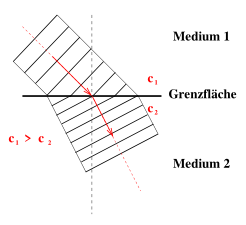
\includegraphics[width=0.35\textwidth]{latex/images/T1.PNG}
        \caption{Schema der Brechung mit Ausbreitungsgeschwindigkeiten\protect \cite{V400}.}
    %    \label{img:schem}
    \end{figure}

    \noindent Für den Fall, dass ein Material Luft ist, wird $n_2$ der Brechungsindex des anderen Mediums als $absolut$ bezeichnet. Werden zwei 
    Materialien verglichen, wird das Material mit höherer Ausbreitungsgeschwindigkeit als \textit{optisch dichter} bezeichnet, anders herum wird das 
    Material als \textit{optisch dünner} bezeichnet. Im Bereich der Strahlenoptik bzw. \textit{geometrischen Optik} sind Lichtstrahlen innerhalb eines 
    homogenen Mediums immer geradlinig und unterschiedliche Strahlen interferieren nicht miteinander.

    \subsection{Reflexion}

        \noindent Wird ein Lichtstrahl an einer ebener Fläche reflektiert, so ist nach dem Reflexionsgestz der Einfallswinkel $\alpha_1$ gleich dem
        Reflexionswinkel $\alpha_2$.

        \begin{figure}[H]
            \centering
            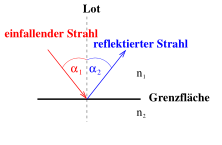
\includegraphics[width=0.35\textwidth]{latex/images/T2.PNG}
            \caption{Schema der Reflexion\protect \cite{V400}.}
        %    \label{img:schem}
        \end{figure}

    \subsection{Brechung}

        \noindent Beim Auftreffen auf ein Medium mit einem anderem Brechungsindex $n$ wird der Lichtstrahl unter einer Richtungsänderung 
        gebrochen. Diese Brechung erflogt nach dem Gesetz von Snellius:

        \begin{equation}
            n_1 \text{sin} \alpha = n_2 \text{sin} \beta
        \end{equation}

        \begin{figure}[H]
            \centering
            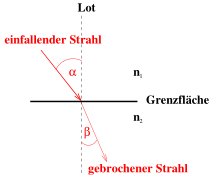
\includegraphics[width=0.35\textwidth]{latex/images/T3.PNG}
            \caption{Schema der Brechung\protect \cite{V400}.}
        %    \label{img:schem}
        \end{figure}

    \subsection{Reflexion und Transmission}

        \noindent Im Normalfall wird ein Lichtstrahl weder komplett gebrochen noch komplett reflektiert, in der Regel wird ein Teil der Intersität 
        transmitiert und ein Teil gebrochen, insgesamt ergeben die Intensitäten dieser beiden Teile aber wieder die Intensität des einfallenden 
        Strahls.

        \begin{figure}[H]
            \centering
            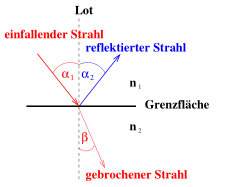
\includegraphics[width=0.35\textwidth]{latex/images/T4.PNG}
            \caption{Schema der Reflexion und Transmission\protect \cite{V400}.}
        %    \label{img:schem}
        \end{figure}

    \subsection{Wellenoptik}
        
        \noindent Die $Strahlenoptik$ ist aber nicht in der Lage einige Phänomene wie zum Beispiel die $Beugung$ zu erklären, diese ist zu 
        beobachten wenn sich Licht in einen Schattenraum ausbreitet. Um die $Beugung$ zu erklären muss mit der $Wellenoptik$ argumentiert werden.\\
        In diesem Bereich besitzten Wellen eine Frequenz $\nu$, die Ausbreitungsgeschwindigkeit $v$ und somit auch eine Wellenlänge $\lambda$.
        Mehrere Wellen interferieren jetzt miteinander, das Bedeutet, dass sich die Gesamtintensität der Wellen an einem Punkt aus der Summe der 
        Einzelintensitäten berechnet ($Superpositionsprinzip$). Sind unterschiedle Wellen aus der gleichen Frquenz und dem gleichen Phasengang 
        aufgebaut, erzeugen sie ein so genanntes $Interferenzbild$. Bei Interferenz wird zwischen $konstruktiver$ und $destruktiver$ Interferenz 
        unterschieden, haben zwei Wellen gleicher Frequenz und Intensität genau einen $Gangunterschied$ von $\lambda$/2, so können sie sich 
        komplett auslöschen.\\
        In diesem Versuch wird die $Beugung$ an einem Gitter genauer untersucht, hier ist wichtig, dass die Dimensionen dess Gitters klein im 
        Vergleich zur Wellenlänge des Lichts sind. Hier besagt das \textit{Huygensche Prinzip} 'Jeder Punkt einer Welle ist der Ausgangspunkt einer 
        Elementarwelle gleicher Frequenz. Die Einhüllende aller Sekundärwellen stellt zu einem spätere Zeitpunkt die neue Lage der Wellenfront
        dar' \cite{400}.\\
        Das einfachste Beispiel hierzu ist der Einzelspalt. Trifft monochromatisches Licht, also eine ebene Wellenfront gleicher Phase auf den 
        Spalt der Breite $a$ wird das Licht nach dem \textit{Huygensche Prinzip} in allen Punkten des Spalts das Licht gebeugt. Die neuen Wellenfronten 
        haben dann dieselbe Frequenz und einen feste Phasenbeziehung. In einem Abstand $L$ wird dann auf einem Schirm das Interferenzbild gemessen. 
        Jediglich die Intensitätsmaxima werden jetzt in diesem Versuch weiter beachtet, diese werden dann durch 

        \begin{equation}
            a \, \text{sin} \alpha = k \lambda
        \end{equation}

        \noindent
        beschrieben. Hier beschreibt $\alpha$ den Winkel zur geradlinigen Ausbreitung des k'ten Intensitätsmaxima bei einem Einzelspalt der breite a 
        und einer Wellenlänge $\lambda$.\\
        Analog lässt sich ein Gesetz für ein Strichgitter aus N-Einzelspalten aufstellen:

        \begin{equation}
            d \, \text{sin} \alpha = k \lambda.
        \end{equation}

        \noindent Hier ist nun $d$ die Gitterkonstante 
        